\chapter{Methodology} \label{methodology}
The purpose of investigating how developers use \gls{gpt} for their projects is to gain the necessary knowledge of the roles chatbot plays in developer-bot collaboration in order to enhance its ability to help developers with their requests. In order to extract the knowledge we firstly cleaned the data, investigated what it consists of and applied topic modelling and sequence mining in order to extract the patterns from developer-chatbot collaboration. 

\section{Data} \todo{discuss that DevGPT dataset was extended with more data}
To answer the research question we have used DevGPT dataset~\cite{devgpt}, which consists of the \gls{gpt} conversations that were shared on GitHub and Hacker News between late May 2023 and the 12th of October 2023. The dataset consists of 9 snapshots (latest: 12th of October, 2023), and each snapshot contains the links collected from GitHub commits, issues, discussion, pull requests, code files, and Hacker News (HN) articles. In this research we use the data from all of the available snapshots. However, to keep the data clean, we remove all the duplicate data based on the shared \gls{gpt} conversation links. Table~\ref{table:data_stat} shows the number of conversations that is left after all the duplicates were removed from the dataset (\textit{DR} row).

\begin{table}[h]
    \centering
    \begin{tabular}{|l|l|l|l|l|l|l|}
         \hline
        & Commits & Issues & Discussions & Pull req. & Code files  & HN  \\
         \hline
        DR & 670 & 516 & 59 & 268 & 2010 & 322\\
         \hline
        NE & 659 & 433 & 51 & 227 & 1616 & 290\\
        \hline
    \end{tabular}
    \caption{Number of conversations after all the duplicates (DR) and non-English conversations (NE) were removed from the data.}
    \label{table:data_stat}
\end{table}

\section{Data cleaning}
At the initial investigation of the data, we discovered that the data contains some information that is not needed to answer the research question of this paper (further referred to as "noise"). Firstly, we only focus on conversations in English, while the dataset contains other languages used for communication with \gls{gpt}. Secondly, in addition to natural language, the prompts  contain program code as a part of the prompt text. Both these factors make the data noisy and require to be dealt with before the data exploration and RQ answering is done. 

\subsection{Language detection}
For the language detection purposes we have used existing libraries: \textit{langdetect\footnote{\url{https://pypi.org/project/langdetect/}}} and \textit{pycld2 (Compact Langauge Detect 2)\footnote{\url{https://pypi.org/project/pycld2/}}}. These two libraries are used to ensure higher accuracy at language detection: if one of the libraries is unable to detect the language, then the other library results influence the decision whether to keep the prompt (if it is detected as English text) or discard. 

For language identification process the prompt is divided into lines and the language is identified for each line. If the line consists of the programming code only, then the line is marked as program (details in Section~\ref{sec:prog-identification}) and the language identification is skipped for this line. This is done in order to avoid prompts in non-English language containing a lot of code lines, which have a lot of English words/keywords, to be identified as an English prompts. The result or language check is a tuple, where the first value is the language identification result of \textit{langdetect} and the second value is \textit{pycld2} result. If the mode language of all the prompt lines is either $("en", "en")$, $("en", "un")$ or $("un", "en")$, then the language of the prompt is considered to be English. Any other language detection result leads to the prompt being discarded. 

\subsection{Program lines detection and its accuracy} \label{sec:prog-identification}
Initially we tried to implement the programming language detection using Guessland python library\footnote{\url{https://pypi.org/project/guesslang/}}, but its accuracy and recall were very low for the dataset that we are using. So it was decided to implement our own code for detecting programming lines in order to remove them before the data analysis is conducted. 

In order to detect the code parts in the prompts, we split all the prompts into lines at line break (\textit{\textbackslash n}) and used the script to detect the probability of the line being a part of code or not. This is done with the assumption that the code blocks are most likely to be present on the separate lines from the natural language sentences and that the code is likely to be spread over multiple lines of the prompt. Thus, the code identification needs to be performed on each line of the code block. If the line contains a code snippet among natural language text, but the natural language part is longer than the code snippet, then the line is identified as a natural language line. In order to detect if the line is programming language or not, we created the function that assigns the line structures (tokens or sentences) with the number that represents how likely the structure is natural language: 0 - programming language, 0.5 - can be either, 1 - natural language. The list below shows what kind of structures are considered in this script:
\begin{itemize}
    \item Line starts with \texttt{//} or \texttt{/*} (C-lamguages, Java, etc.), \texttt{--} (Haskell), \texttt{\#} or \texttt{"""} (Python), \texttt{<!--} (HTML) or ends with \texttt{*/}, \texttt{"""} or \texttt{-->} indicates that the line is a part of comment within the program (likelyhood: 0);
    \item Line starts opening HTML tag (e.g. \texttt{<p>}, \texttt{<h1>}, etc.) and ends with closing HTML tag (e.g. \texttt{</p>}, \texttt{</h1>}, etc.) indicates that the line is a part of HTML code (likelyhood: 0);
    \item Structure is a keyword in Java, C (C++, C\#), HTML, CSS, Python, Command Prompt or Linux command (likelyhood: 0.5);
    \item Structure is upper case (also covers SQL keywords) (likelyhood: 0.5);
    \item Structure is written in camel or pascal case (likelyhood: 0);
    \item Structure only consists of letters (likelyhood: 1);
    \item Structure consists of letters and comma, period, colon, question or exclamation mark (likelyhood: 0.5);
    \item Structure is a word surrounded with square brackets (likelyhood: 0);
    \item Structure has no letters or is empty string (likelyhood: 0);
    \item Structure starts with $::$, $::-$, $:$, $\#$, $.$, $<\backslash \backslash$, $<$ followed by a word (likelyhood: 0);
    \item Structure is a word surrounded with less-that and greater-than signs (likelyhood: 0);
    \item Structure is a combination of two words with a dot in between (likelyhood: 0);
    \item Structure has a form of function or function call: $function\_name(args)$, where $args$ is a list of 0 or more arguments separated by the comma (likelyhood: 0);
\end{itemize}

The likelihood of line having a natural language text in it is calculated by summing all the likelyhoods together and dividing by the number of structures in the line. If the result is abive 0.5, the line is considered to contain the natural language text in it, if the likelyhood is lower, then the line is most likely the code line. 

The usability of the program code detection script is tested using 5 randomly selected conversations and taking up to 20 randomly selected lines out of these 5 conversations. The selected lines are sent to the script and the script results were saved into the file, where the line content was manually evaluated to be the program code or not. The results of the script performance were satisfactory for all the conversation sources:
\begin{itemize}
    \item GitHub commits: 5 false-positives and 2 false-negative (accuracy: 0.88, F1-score: 0.9;
    \item GitHub issues (accuracy: 1, F1-score: 1);
    \item GitHub discussions: 1 false-positives and 0 false-negative (accuracy: 0.99, F1-score: 0.98); 
    \item GitHub pull requests: 1 false-positives and 1 false-negative (accuracy: 0.95, F1-score: 0.97); 
    \item GitHub code files: 2 false-positives and 0 false-negative (accuracy: 0.97, F1-score: 0.98);
    \item Hacker News (accuracy: 1, F1-score: 1);
\end{itemize}

The false-positive and false-negative results are printed out to inspect what mistakes are made by the written script. Most common mistakes are HTML and SQL code lines that are marked as "not a code", due to the high number of natural language structures they contain. For example, HTML paragraphs \texttt{<p>} contain whole sentence(s) written in natural language, which influence the final result of the script. Sentences containing high number of punctuation marks, on the other hand, are often marked as the program, even when they are not. For example, lines \textit{"perfect!"} and \textit{"- Prefer *async/await* over promises!"} were predicted to be a program, however, it can also be a part of text. Despite that, the results of the script are on average above 85\% accuracy and F1 score, which we consider to be a good result for this research. 

\section{Data exploration}
As a part of data exploration, we focus on gathering some statistics about the data set: how long the conversations are, how many symbols or words is each prompt on average, the most common n-grams and topics that can be extracted from the prompts. 

Before going into discussion about the statistics of the data collected, it is important to explain some vocabulary used in this section. Users write \textit{prompts} to \gls{gpt}, which uses them to formulate the answer. The collection of such prompt-answer pairs that happens in the same conversation thread is called \textit{conversation}. In this dataset we only focus on the prompts written by the user and discard the answers generated by \gls{gpt} in all the conversations. 

\subsection{Statistics and outliers}
This section covers some statistics regarding the length of the conversations and prompts and the outliers encountered during data exploration process. 

\subsubsection{Number of prompts in conversations}
The number of prompts in the conversations varied significantly for the conversations obtained from the different sources. The shortest conversations were found at GitHub discussion dataset, while GitHub code files dataset contained longest discussions among all the datasets. Table~\ref{table:conv-lengths} shows the statistics of the conversation lengths for every dataset obtained from different sources. The median conversation length values for all the conversation sources are similar to each other, staying between 1 and 7 prompts per conversations. But when it comes to the mean and standard deviation, the difference becomes more significant. GitHub commits, issues and code files related conversations are considerably longer than the conversations from the other sources. This can be concluded from the higher mean of 23.1, 21.7 and 22.6 prompts and very high standard deviations of 85.4, 59.4 and 100.5 prompts for GitHub commits, issues and code files, respectively. These high numbers are mainly influences by the outliers present in these datasets that are discussed later in this section. The other datasets had lower mean and standard deviation values, where mean and standard deviation seem to represent the data quite well.

\begin{table}[H]
\centering
\begin{tabular}{l||c|c|c}
Source           & Median & Mean & Standard deviation \\ \hline
GH Commits       & 2      & 23.1 & 85.4               \\
GH Issues        & 3      & 21.7 & 59.4              \\
GH Discussions   & 3      & 6.7  & 10.4               \\
GH Pull requests & 1      & 4.9  & 19.9               \\
GH code files    & 5      & 22.6 & 100.5              \\
HackerNews       & 7      & 17.6 & 40              
\end{tabular}   
\caption{Median, mean and standard deviation of the conversation lengths from different sources.}
\label{table:conv-lengths} 
\end{table}

Figure~\ref{fig:conv-per-prompt} contains plots where the line shows how many conversations are there per number of the prompt. Axis \textit{x} represents the prompt number, where minimum value is 1 and maximum value is the number of prompts in the longest conversation of this dataset. Axis \textit{y} shows how many conversations have \textit{x} or more prompts at any \textit{x}-value. The figure shows that all the conversations sources from GitHub have some conversations that are significantly longer than the rest of the conversations in the dataset. A good example is one conversation from pull requests, that is about 133 prompts longer than the next longest conversation in this dataset. The conversations that seemed to be outliers in each of the datasets were saved to the file for the further investigation of their content. In each dataset there were conversations, which prompt numbers are much greater that the prompt numbers of the next longest conversations. In order to capture them, we have selected the following cut-off points for the conversation lengths, and saved the ones that were longer or equal to these points: 
\begin{itemize}
    \item GitHub commits: conversation length of 30 or more;
    \item GitHub issues: conversation length of 30 or more;
    \item GitHub discussions: conversation length of 15 or more;
    \item GitHub pull request: conversation length of 30 or more;
    \item GitHub code files: conversation length of 100 or more;
    \item Hacker News: conversation length of 50 or more;
\end{itemize}

\begin{figure}[H]
    \centering
    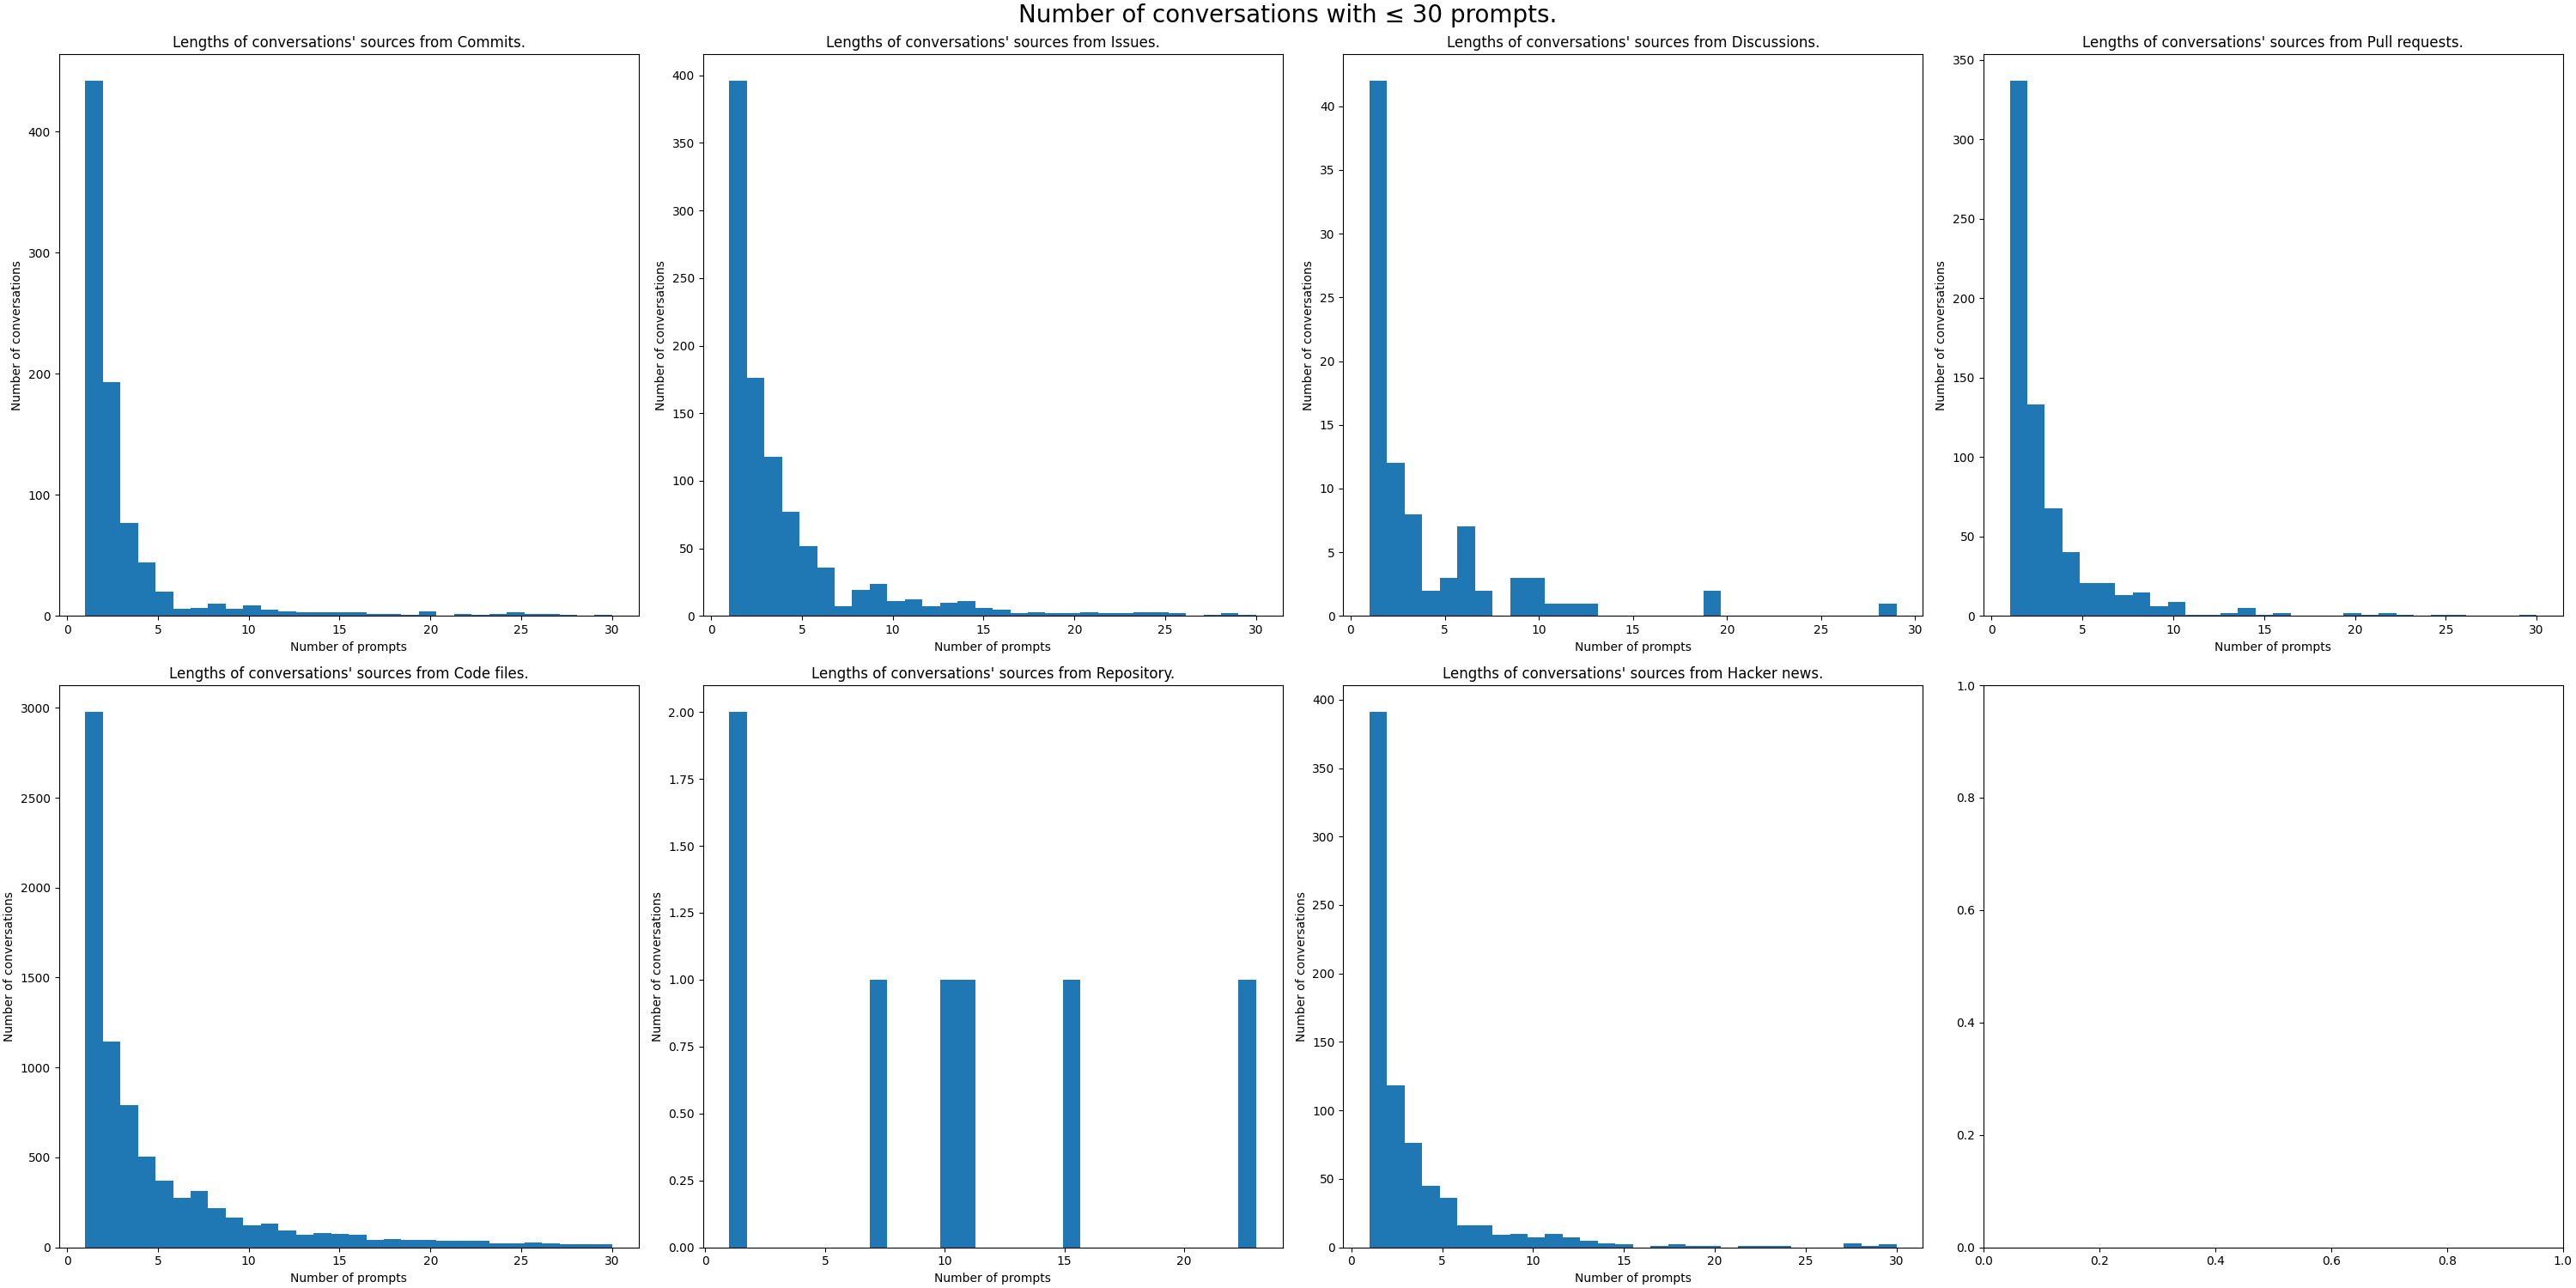
\includegraphics[width=\textwidth]{imgs/conv-per-prompt-nr.png}
    \caption{Number of conversations per prompt number for all conversation sources.}
    \label{fig:conv-per-prompt}
\end{figure}

\subsubsection{Outliers and their content}
The conversations that are too long are saved to the file and investigated manually for the reasons why they contain that many prompts. Doing that we managed to find the following reasons on why they were that long:
\begin{itemize}
    \item Conversation contains several prompts of text that did not fit into one prompt due to the set character limit: users were copying the whole code files, articles or books.
    \item Users were asking for code snippets, and the code provided from \gls{gpt} either did not correspond to user expectations and the request had to be modified several times by the user, or the code returned the errors, that users were not able to solve and had to ask for help from \gls{gpt}.
    \item Users used \gls{gpt} for programming: they provided with the information what they want it to program, asking \gls{gpt} to write the code, while testing it on their machine and providing with the feedback on the errors received or what needs to be changed.
    \item Users use \gls{gpt} as their mentor: they post the code they wrote asking for explanation or improvements suggestions. Occasionally posting errors it produced and asking for help or explanation.
    \item Users use \gls{gpt} for conversations that are not related to the programming issues: talking about \gls{gpt} opinions on different topics, asking for advice or asking more general questions; 
\end{itemize}

\subsubsection{Average symbol/word count per prompt}
The number of symbols and words per prompts varied significantly depending on the source of the conversation. However, the graphs for the number of symbols and the number of words per each source are comparable, where the peaks and troughs on the graphs are present at the same locations. Thus, we will look at both the number of symbols and the number of words together to investigate the outliers that have too high symbol/word count.

Figure~\ref{fig:symbols-per-prompt} and \ref{fig:words-per-prompt} show the average number of symbols and words per current prompt number, respectively. Axis \textit{x} represents the prompt number, where minimum value is 1 and maximum value is the number of prompts in the longest conversation of this dataset. Axis \textit{y} shows the average count of symbols/words that prompt \textit{x} has. One important factor that influences the way graphs look like is the length of conversations. The graphs show average count of symbols/words for the prompt number: some conversations are shorter than others, meaning that longer conversations have more influences on the average symbol/word count for the higher prompt counts, since the average is calculated on the lower number of prompts. A good example of it is GitHub discussion dataset, which has only one conversation longer than 19 prompts, meaning that the average symbol/word count for prompts 20 to 29 is taken from one conversation, which results in peaks on the graphs. GitHub code files dataset shows different behaviour: longest conversations have lower symbol/word counts. However, in all datasets first prompts are usually used to introduce the problem \gls{gpt} needs to solve, which requires a more thorough description of the problem; thus, resulting in a higher symbol/word count.

To investigate the outliers, we have selected the cut-off points for each dataset separately. The cut-off point is selected to be 2/3 of the maximum average. Conversations containing prompts longer than the cut-off points were saved for the further investigation. GitHub commits and HackerNews datasets have smooth graphs with little fluctuation, thus, they are not included in outlier investigation process. For all the other four datasets we have selected the following cut-off points:
\begin{itemize}
    \item GitHub issues: prompt length in symbols of 400 or more;
    \item GitHub discussions: prompt length in symbols of 800 or more;
    \item GitHub pull request: prompt length in symbols of 800 or more;
    \item GitHub code files: prompt length in symbols of 850 or more;
\end{itemize}

\begin{figure}[H]
    \centering
    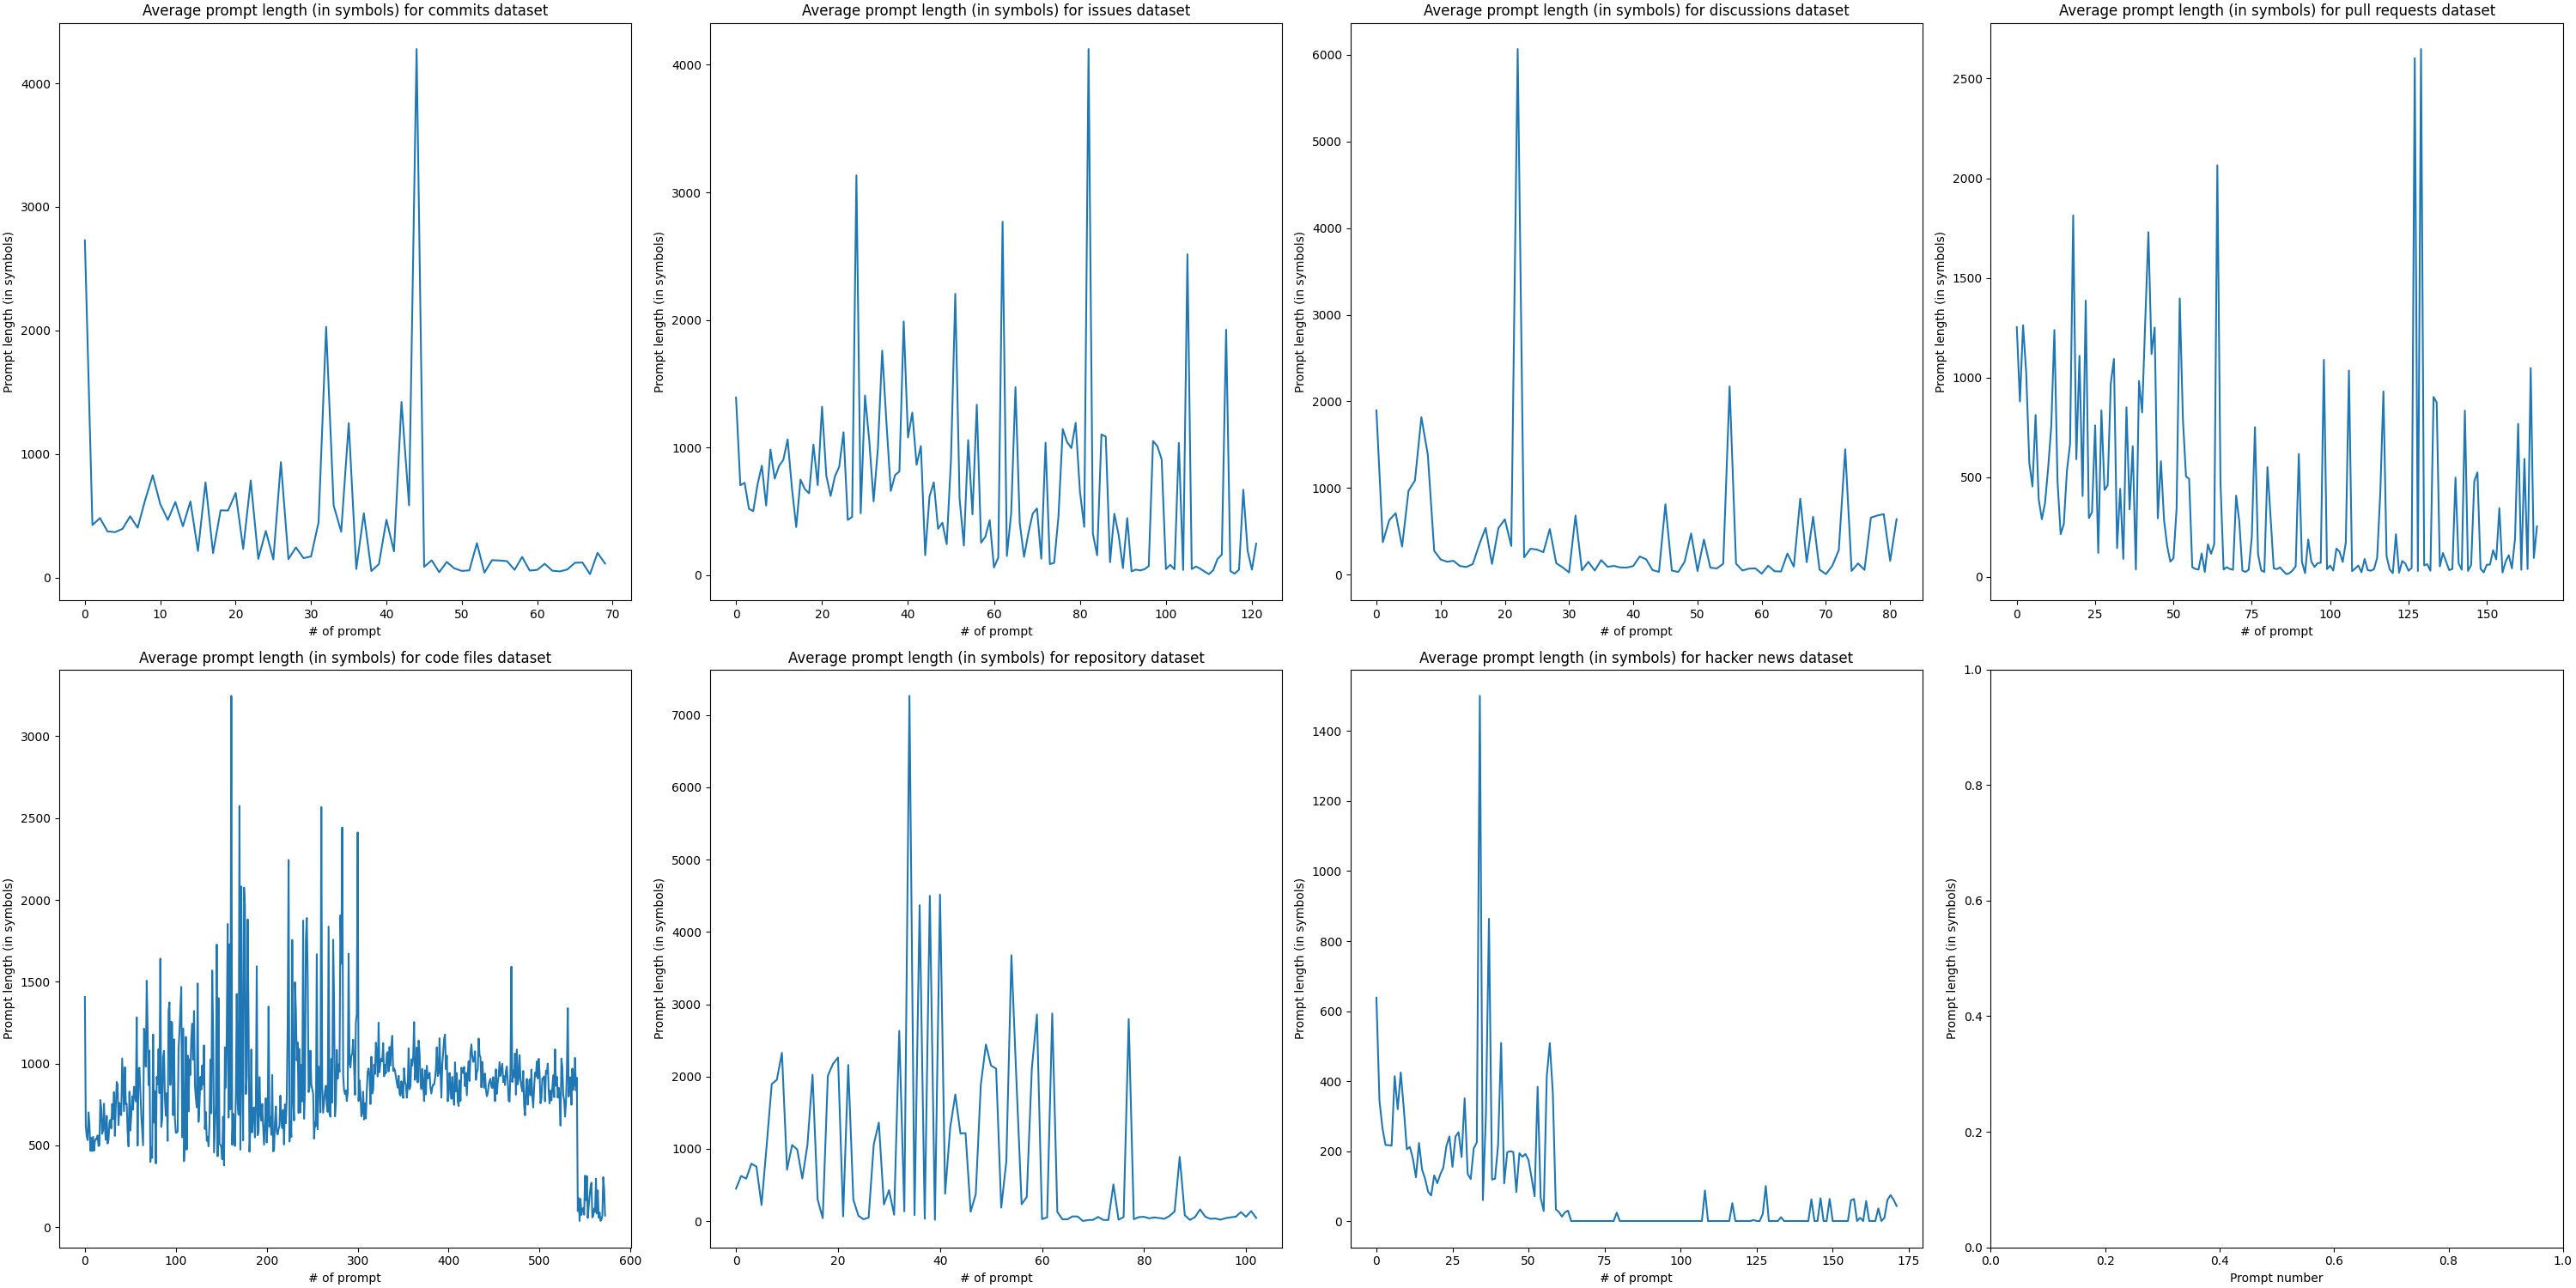
\includegraphics[width=\textwidth]{imgs/symbols-per-prompt.png}
    \caption{Average symbol count per prompt number for all conversation sources after code lines were removed.}
    \label{fig:symbols-per-prompt}
\end{figure}

\begin{figure}[H]
    \centering
    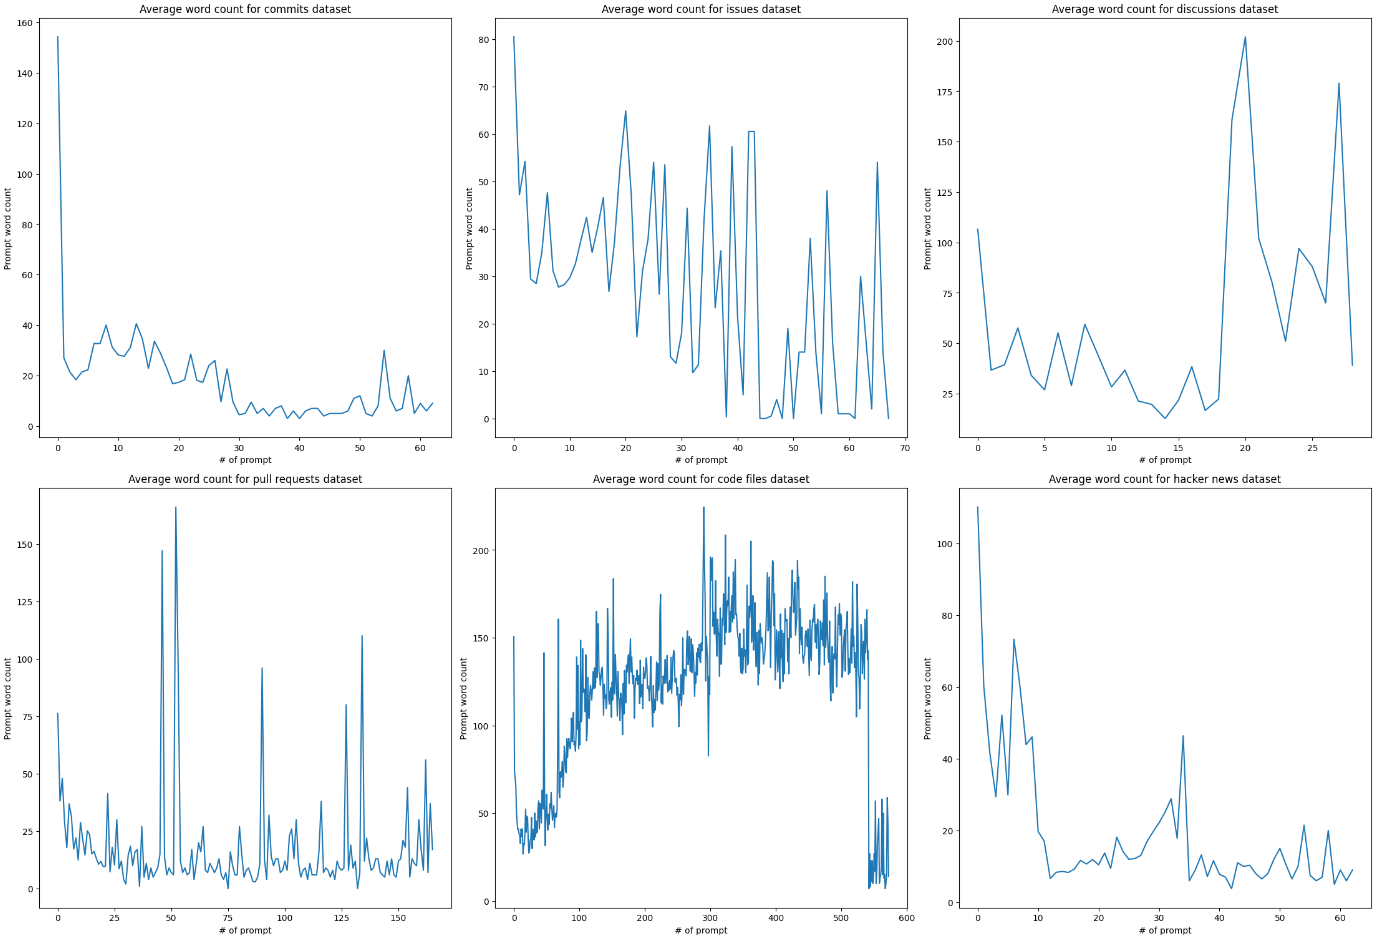
\includegraphics[width=\textwidth]{imgs/word-count-per-prompt.png}
    \caption{Average word count per prompt number for all conversation sources after code lines were removed.}
    \label{fig:words-per-prompt}
\end{figure}

\subsubsection{Outliers and their content}
The conversations containing very long prompts are saved to the file, and their content is investigated manually to identify the reasons that explain their length. We have managed to identify the following content categories in long prompts:
\begin{itemize}
    \item Prompt contains long text that was pasted by the user from the external source (scientific article, GitHub issue description, code documentation, etc.), and user wants to get the analysis or explanation of the text or its part, or wants to get the rewritten version to match the target audience.
    \item Prompt contains error message, code documentation/comments and code parts (that were not detected by program line detection function) that user wants to fix, debug, get feedback on.
    \item Prompt contains a thorough description of the problem the user is facing, which can contain:
    \begin{itemize}
        \item A very detailed problem description, when the user knows exactly what they want to receive from \gls{gpt};
        \item A problem description in a poetic way (usually asking \gls{gpt} to play a certain role: e.g. teacher, mentor, area expert);
        \item User provides relevant for the problem background information to \gls{gpt};
        \item Multiple questions regarding the problem or provided solution; 
        \item What solutions user found, which did not work;
        \item Long URL links;
        \item The list of requirements or instructions;
        \item Example of the output, functionality, or code user wants to receive.
    \end{itemize}
\end{itemize}

\section{Data preparation} \label{sec:data-prep}
In order to perform further analysis, we have pre-processed the remaining data using lemmatisation and tokenisation processes.  

During lemmatisation process we split sentences into a list of structures: words, punctuation, digits or alphanumeric values; and lemmatise them using \textit{lemmatize\_sentence} function from \textbf{pywsd} package~\cite{pywsd14}. The function tries to convert a surface word into lemma, and if lemmatize word is not in wordnet then try and convert surface word into its stem. 

Once all the sentences are lemmatised, they are cleaned from the non-relevant data. We remove the following tokens: 
\begin{itemize}
    \item Links: token starts with \textit{"http"};
    \item Stop words: the selection of \textit{stop\_words} from \textbf{nltk} package\footnote{\href{https://www.geeksforgeeks.org/removing-stop-words-nltk-python/}{Stop words list}}~\cite{nltk};
    \item Punctuation; 
    \item Word contains digits.
\end{itemize}

Lemmatised and cleaned lists of tokens are then further passed on to the functions that conduct further analysis on the content of the cleaned sentences. 

\section{N-grams}
N-grams is a sequence of \textit{n} consecutive characters, words or other textual structures~\cite{n-grams}, where \textit{n} is the number of such structures in a pair. The set of n-grams is obtained by shifting the box of \textbf{n} structures through the data and retrieving the values. The structures order is kept when the n-grams are being extracted. In this research we focus on the words, so the sentence \textit{"That fox is chasing a rabbit"} can be split into the following structures: ${that, fox, is, chasing, a rabbit}$. We can create the following n-grams from the mentioned set of words:
\begin{itemize}
    \item Bi-grams: $(that, fox)$, $(fox, is)$, $(is, chasing)$, $(chasing, a)$, $(a, rabbit)$; 
    \item Tri-grams: $(that, fox, is)$, $(fox, is, chasing)$, $(is, chasing, a)$, \\$(chasing, a, rabbit)$;
    \item Quadri-grams: $(that, fox, is, chasing)$, $(fox, is, chasing, a)$, \\$(is, chasing, a, rabbit)$;
\end{itemize}

Before the data is used for n-grams extraction, the data is cleaned from stop words, as described in Section~\ref{sec:data-prep}. In the example above it would mean that words \textit{"that"}, \textit{"is"} and \textit{"a"} will be removed in the pre-processing step. All the other context carrying words are used to create n-grams for the data. N-grams are created using \textit{ngrams()} function from \textbf{nltk} package, where \textit{n} is set to the desirable value. The extracted n-grams are used to create n-grams frequency distribution: all the same n-grams are grouped together and their frequency is calculated. Such frequency distribution allows us to order all the extracted n-grams in descending order based on their frequency and focus our analysis on the most frequent n-grams. 

For easier visualisation, we use WordCloud package~\cite{wordcloud} that generates word clouds where the most common n-grams use bigger font size, while less common ones use smaller font sizes that is dependent on their frequency.

\section{Topic modelling}
Topic models are generative models that provide a probabilistic framework~\cite{topic-model}. These models are used for large electronic text collections to organise, understand, search and summarise their content. 

The topics are the relations that link words in a vocabulary and their occurrence in documents. Each document is viewed as a mixture of topics. Topic models discover different themes present in the text collections and annotate the documents according to the themes. The document coverage distribution of topics is then generated to provide an overview of topics found in this document collection. 

In this study we use \gls{lda} topic modelling -- one of the most popular text modelling techniques. \gls{lda} is a probabilistic generative model that allows the observations to be described by unobserved data that explains why some parts of the data are similar to each other~\cite{tong-topic-modelling}. In \gls{lda}, documents consist of multiple topics and each topic is a distribution over a fixed vocabulary. For example, if we have the  following vocabulary of \{\textit{pan, cook, football, basketball}\}, then the kitchen topic will assigne high probabilities to the words \textit{pan} and \textit{cook}, while \textit{football} and \textit{basketball} will have very low probabilities; however, the sport topic will have the opposite probabilities for all the words. 

In the implementation we use the data cleaned in the pre-processing step as described in Section~\ref{sec:data-prep}. We start with creating the vacabulary: this is done using \textit{CountVectorizer} class to convert a collection of text documents to a matrix of token counts~\cite{scikitlearnCountVectorizer}. The parameters of \textit{min\_df} and \textbf{max\_df} are set to 0 and 1 respectively; \textit{ngram\_range} is set to tuple of (1,4), making vocabulary to consist of n-grams of the length 1 to 4 words; and the stop words are the stop words from \textbf{nltk} package. For topic modelling we use \textit{LatentDirichletAllocation} class from \textbf{sklearn} package~\cite{scikitlearnLatentDirichletAllocation}\todo{Code: remove split, use fit\_transform}, where we set number of topics to 10, iteration count to 6 and random state to 42. We calculate perplexity and coherence score of the topic model and visualise them along with WordCloud visualisation of the topics. 

\section{Sequence mining}
\todo{add}

\section{Limitations}
There exist limitations of the dataset and methods selected for this study that influence the results of the research. These limitation are addressed in this section. 

Dataset used for this study provides a good overview of how developers use \gls{gpt} for solving their daily problems. However, the sources that were used to extract this knowledge are not completer. The conversation data was collected from GitHub (commits, code files, discussions, pull requests and issues) and HackerNews, and it covers the conversations that happened between the release date of \gls{gpt} and 12th of October 2023. Thus, the data is not complete and misses other sources that could contain more knowledge regarding the use of \gls{gpt} by developers. Additionally, since the data was last sourced over a year ago, the conversations that happened after the mentioned date and conversations with \gls{gpt} that uses newer version GPT-4\footnote{\url{https://openai.com/index/gpt-4/}} are not included in this dataset. Moreover, some conversation links that were used to scrape the data are not working anymore, thus, the validity of these conversations cannot be checked.

Additionally, the language detection tool and the data cleaning method used are not fully accurate and miss prompts or prompt lines that contain foreign language and code. It was discovered, that the prompts often contain pasted text (articles, documentation, code comments) and error messages, which are hard to detect using the selected tool set, since they contain sentences in natural English language, but do not contain the information needed for answering the research question. Thus, the code snippets, foreign language prompts and copied texts add noise to the data that the tools are not able to detect.